\documentclass{mycworkshop}

\usepackage{tabularx}
\usepackage[gray]{xcolor}
\usepackage{tikz}
\usetikzlibrary{mindmap}

% bibliography set up
\usepackage[style=sbl]{biblatex}
\usepackage{filecontents}
\begin{filecontents}{\jobname.bib}
@book{roberts:2002,
  author = {Roberts, Vaughan},
  title = {God's Big Picture},
  subtitle = {Tracing the Storyline of the Bible},
  location = {Nottingham},
  publisher = {Inter-Varsity},
  date = {2002},
  addendum = {\mkbibparens{Also available in Chinese \mkbibparens{Traditional Script}}}
}
@book{lloyd-jones:2015,
  author = {LLoyd-Jones, Sally},
  title = {The Story of God's Love for You},
  location = {Grand Rapids},
  publisher = {Zondervan},
  date = {2015}
}
\end{filecontents}
\addbibresource{\jobname.bib}

\begin{document}

\title{}
\subtitle{FOCUS on Jesus: Making Sense of the Whole Bible}
\maketitle

\question*{Q. What do you find difficult about reading the Bible?}

\medskip

\subsection*{The Bible: God's big picture for the world}

A unifying theme: The kingdom of God.

\begin{quote}[Vaughan Roberts, \emph{God's Big Picture}, p.22]
  “God's people in God's place under God's rule and blessing.”
\end{quote}

\smallskip

\subsection*{One book, one author, and one subject}

God's wonderful plan to \hrulefill .

\smallskip

\section{The Pattern of the Kingdom: Creation}

\pbibleverse{Gen 1:26-27; 2:1-3, 7-9, 15-17}

\begin{tabularx}{\linewidth}{|>{\itshape}l|X|}
  \hline
  People & \\[10.8bp]
  \hline
  Place & \\[10.8bp]
  \hline
  Rule \& Blessing & \\[10.8bp]
  \hline
\end{tabularx}

\section{The Perished Kingdom: Fall}

\begin{tabularx}{\linewidth}{|>{\itshape}l|l|X|}
  \hline
  People & \pbibleverse{Gen 3:19} & \\[10.8bp]
  \hline
  Place & \pbibleverse{Gen 3:23} & \\[10.8bp]
  \hline
  Rule \& Blessing & \pbibleverse{Gen 3:6, 17} & \\[10.8bp]
  \hline
\end{tabularx}

\begin{description}
  \item[Fulfilment in Jesus:] He comes as the serpent crusher
    (\pbibleverse{Gen 3:15; 1 John 3:8})
\end{description}

\smallskip

\begin{description}
  \item[Fulfilment in Jesus:] He is like Adam, but better (\pbibleverse{Rom
    5:19; 1 Cor 15:20-22})
\end{description}

\section{The Promised Kingdom: Abraham}

\pbibleverse{Gen 12:1-4}

\begin{tabularx}{\linewidth}{|>{\itshape}l|X|}
  \hline
  People & \\[10.8bp]
  \hline
  Place & \\[10.8bp]
  \hline
  Rule \& Blessing & \\[10.8bp]
  \hline
\end{tabularx}

\begin{description}
  \item[Fulfilment in Jesus:] He is the one through whom blessing flows to all
    nations (\pbibleverse{Gal 3:14})
\end{description}

\section{The Partial Kingdom: Covenant with Moses; Covenant with David}

\subsection{Exodus}

\begin{indentblock}
  Slavery and deliverance at Passover (\pbibleverse{Exod 6:6-8; 12:21-22;
  14:29-30})

  \vfill

  \begin{description}
    \item[Fulfilment in Jesus:] He is the Passover lamb who was sacrificed for
      us (\pbibleverse{1 Cor 5:7})
  \end{description}
\end{indentblock}

\vfill

\subsection{Living under God}

\begin{indentblock}
  Covenant through the Law (\pbibleverse{Exod 19:4-6})

  \vfill

  Tabernacle (\pbibleverse{Exod 25:8})

  \vfill

  Land (\pbibleverse{Josh 23-24})

  \vfill

  \begin{description}
    \item[Fulfilment in Jesus:] God is with us in Jesus (\pbibleverse{Matt
      1:21-23})
  \end{description}
\end{indentblock}

\vfill

\subsection{Judges and Kings}

\begin{indentblock}
  David (\pbibleverse{2 Sam 7:8-16})

  \vfill

  \begin{description}
    \item[Fulfilment in Jesus:] He will rule on David's throne forever
      (\pbibleverse{Luke 1:30-33})
  \end{description}
\end{indentblock}

\vfill

\begin{tabularx}{\linewidth}{|>{\itshape}l|X|}
  \hline
  People & \\[10.8bp]
  \hline
  Place & \\[10.8bp]
  \hline
  Rule \& Blessing & \\[10.8bp]
  \hline
\end{tabularx}
\smallskip

\section{The Prophesied Kingdom: Hope of the New Covenant}

\subsection{Israel's decline}

\subsection{Promise of Messiah/servant (\pbibleverse{Isa 53})}

\begin{indentblock}
  \begin{description}
    \item[Fulfilment in Jesus:] He makes a new covenant with us and pours out
      God's Spirit on all God's people (\pbibleverse{Matt 26:28; Acts 2})
  \end{description}
\end{indentblock}

\section{The Present Kingdom: Jesus}

\subsection{Jesus came to fulfil the Old Testament (\pbibleverse{Matt
5:17-18})}

\subsection{Jesus: The centre of God's plans}

\begin{indentblock}
  \begin{center}
    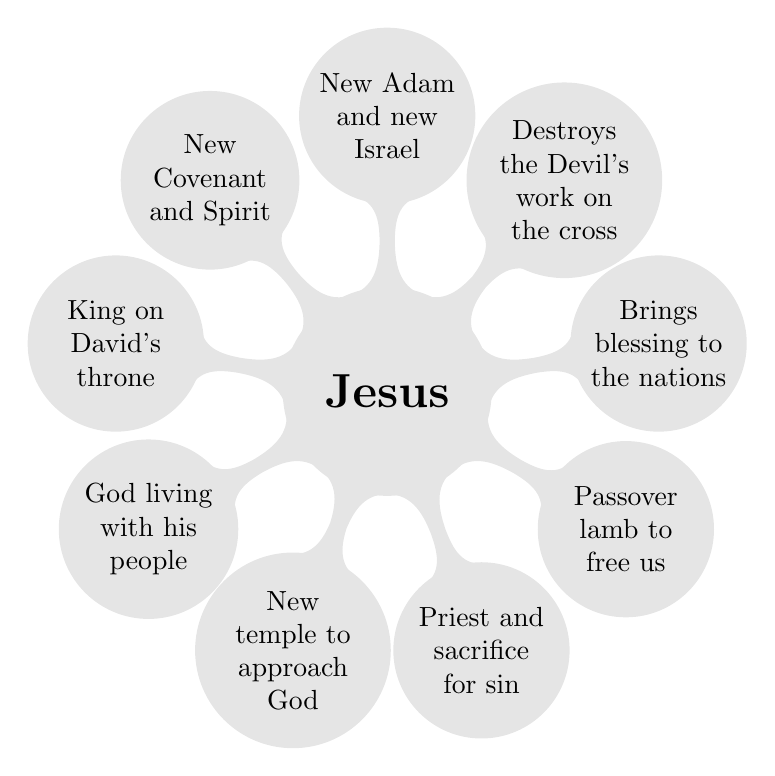
\begin{tikzpicture}[
        mindmap, every node/.style={concept},
        concept color=black!10, grow cyclic,
        root concept/.append style={minimum size=0pt,text width=2.5cm,
          font=\sourcesanspro\fontsize{16.06}{19.34787}\selectfont\bfseries},
        level 1/.append style={sibling angle=40, level distance=3.5cm,
          font=\sourcesanspro, minimum size=1.8cm, text width=1.8cm, clockwise
          from=90}]
      \node [root concept] {Jesus}
        child { node {New Adam and new Israel} }
        child { node {Destroys the Devil's work on the cross} }
        child { node {Brings blessing to the nations} }
        child { node {Passover lamb to free us} }
        child { node {Priest and sacrifice for sin} }
        child { node {New temple to approach God} }
        child { node {God living with his people} }
        child { node {King on David's throne} }
        child { node {New Covenant and Spirit} };
    \end{tikzpicture}
  \end{center}
\end{indentblock}

\begin{tabularx}{\linewidth}{|>{\itshape}l|X|}
  \hline
  People & \\[10.8bp]
  \hline
  Place & \\[10.8bp]
  \hline
  Rule \& Blessing & \\[10.8bp]
  \hline
\end{tabularx}
\smallskip

\section{The Proclaimed Kingdom: The Last Days (Today)}

\begin{tabularx}{\linewidth}{|>{\itshape}l|p{3cm}|X|}
  \hline
  People & \pbibleverse{1 Pet 2:9}; cf.~\pbibleverse{Exod 19:6; Deut 7:6} &
    \\[10.8bp]
  \hline
  Place & \pbibleverse{1 Cor 6:19} & \\[10.8bp]
  \hline
  Rule \& Blessing & \pbibleverse{Rom 3:20; 7:6} & \\[10.8bp]
  \hline
\end{tabularx}

\section{The Perfected Kingdom: New Creation (Future)}

\begin{tabularx}{\linewidth}{|>{\itshape}l|l|X|}
  \hline
  People & \pbibleverse{Rev 7:9; 21:3} & \\[10.8bp]
  \hline
  Place & \pbibleverse{Rev 21:1-4} & \\[10.8bp]
  \hline
  Rule \& Blessing & \pbibleverse{Rev 22:3-5} & \\[10.8bp]
  \hline
\end{tabularx}

\section*{Exercise}

\subsection*{Read \pbibleverse{Judg 3:7-11}}

\begin{quote}
  \textbf{\pbibleverse{Judg 3:7}} The Israelites did evil in the eyes of the
  \textsc{Lord}; they forgot the \textsc{Lord} their God and served the Baals
  and the Asherahs. \vs{8}The anger of the \textsf{Lord} burned against Israel
  so that he sold them into the hands of Cushan-Rishathaim king of Aram
  Naharaim, to whom the Israelites were subject for eight years. \vs{9}But
  when they cried out to the \textsc{Lord}, he raised up for them a deliverer,
  Othniel son of Kenaz, Caleb's younger brother, who saved them. \vs{10}The
  Spirit of the \textsc{Lord} came on him, so that he became Israel's judge
  and went to war. The \textsc{Lord} gave Cushan-Rishathaim king of Aram into
  the hands of Othniel, who overpowered him. \vs{11}So the land had peace for
  forty years, until Othniel son of Kenaz died.
\end{quote}

\question*{Q. How would you read Othniel's story in light of God's picture of
salvation?}

\vfill

\nocite{*}

\printbibliography[title=Book Recommendations]

\end{document}
